\documentclass[12pt,letterpaper]{article}
\usepackage{graphicx,textcomp}
\usepackage{natbib}
\usepackage{setspace}
\usepackage{fullpage}
\usepackage{color}
\usepackage[reqno]{amsmath}
\usepackage{amsthm}
\usepackage{fancyvrb}
\usepackage{amssymb,enumerate}
\usepackage[all]{xy}
\usepackage{endnotes}
\usepackage{lscape}
\newtheorem{com}{Comment}
\usepackage{float}
\usepackage{hyperref}
\newtheorem{lem} {Lemma}
\newtheorem{prop}{Proposition}
\newtheorem{thm}{Theorem}
\newtheorem{defn}{Definition}
\newtheorem{cor}{Corollary}
\newtheorem{obs}{Observation}
\usepackage[compact]{titlesec}
\usepackage{dcolumn}
\usepackage{tikz}
\usetikzlibrary{arrows}
\usepackage{multirow}
\usepackage{xcolor}
\newcolumntype{.}{D{.}{.}{-1}}
\newcolumntype{d}[1]{D{.}{.}{#1}}
\definecolor{light-gray}{gray}{0.65}
\usepackage{url}
\usepackage{listings}
\usepackage{color}

\definecolor{codegreen}{rgb}{0,0.6,0}
\definecolor{codegray}{rgb}{0.5,0.5,0.5}
\definecolor{codepurple}{rgb}{0.58,0,0.82}
\definecolor{backcolour}{rgb}{0.95,0.95,0.92}

\lstdefinestyle{mystyle}{
	backgroundcolor=\color{backcolour},   
	commentstyle=\color{codegreen},
	keywordstyle=\color{magenta},
	numberstyle=\tiny\color{codegray},
	stringstyle=\color{codepurple},
	basicstyle=\footnotesize,
	breakatwhitespace=false,         
	breaklines=true,                 
	captionpos=b,                    
	keepspaces=true,                 
	numbers=left,                    
	numbersep=5pt,                  
	showspaces=false,                
	showstringspaces=false,
	showtabs=false,                  
	tabsize=2
}
\lstset{style=mystyle}
\newcommand{\Sref}[1]{Section~\ref{#1}}
\newtheorem{hyp}{Hypothesis}

\title{Problem Set 1}
\date{Due: October 8, 2026}
\author{Applied Stats/Quant Methods 1}

\begin{document}
	\maketitle
	
	\section*{Instructions}
	\begin{itemize}
	\item Please show your work! You may lose points by simply writing in the answer. If the problem requires you to execute commands in \texttt{R}, please include the code you used to get your answers. Please also include the \texttt{.R} file that contains your code. If you are not sure if work needs to be shown for a particular problem, please ask.
\item Your homework should be submitted electronically on GitHub.
\item This problem set is due before 23:59 on Thursday October 8, 2026. No late assignments will be accepted.
	\end{itemize}
	
	\vspace{1cm}
	\section*{Question 1: Education}

A school counselor was curious about the average of IQ of the students in her school and took a random sample of 25 students' IQ scores. The following is the data set:\\
\vspace{.5cm}

\lstinputlisting[language=R, firstline=36, lastline=36]{PS01_AL.R}  


\vspace{1cm}

\begin{enumerate}
	\item Find a 90\% confidence interval for the average student IQ in the school (As a hint, you first need the mean and SD to create a CI):\\
	
	I started by calculating the sample mean and assigning it to an object. 
\lstinputlisting[language=R, firstline = 39, lastline = 39]{PS01_AL.R}
	Afterwards, I calculate the standard deviation and the stand error.
\lstinputlisting[language=R, firstline = 40, lastline = 45]{PS01_AL.R}

Because our dataset has fewer than 30 observations, we should use the t-distribution to calculate the confidence interval. Therefore, I assigned two objects: the first contains our alpha level of 10 per cent (0.10). The second object contains our degrees of freedom. I used the object n, which I created to calculate the standard error, to calculate the degrees of freedom. This procedure has the (theoretical) advantage that I could rerun the script with fewer adjustments if I obtained additional data.

\lstinputlisting[language=R, firstline = 48, lastline = 49]{PS01_AL.R}

Based on this preparation, I could extract the t-score and use the combined objects to calculate the upper and lower bounds of my confidence interval. Then I combined these two, into one object and printed it out. 

\begin{verbatim}
	> t_score <- qt(p = alpha / 2,
	+               df = degrees_of_freedom, 
	+               lower.tail = FALSE)
	> # Now we can calculate the lower bound & upper bound
	> lower_90 <- sample_mean - (t_score * standard_error)
	> upper_90 <- sample_mean + (t_score * standard_error) 
	> ci90 <- c(lower_90, upper_90)
	> ci90
	[1]  93.95993 102.92007
\end{verbatim}
 
	
	\item Next, the school counselor was curious  whether  the average student IQ in her school is higher than the average IQ score (100) among all the schools in the country.\\ 
	

	\noindent Using the same sample, conduct the appropriate hypothesis test with $\alpha=0.05$.
\end{enumerate}

Our hypthesis test is conducted in five steps.
The first step is to check the assumptions.
We have random data, continous data, and a mean comparison.
However, we have less than 30 observations. Therefore, we use a one sample t-test.

The second step is to formulate our Hypothesis and to set our alpha.
H0: The mean IQ in our sample is equal or less than 100
H1: The mean IQ in our sample is greater than 100. 
As mentioned in the instructions $\alpha = 0.05$


\newpage

The third step is to calculate the test statistic.
The forth step is to calculate the p-Value. R does both in one step: 
By using the t.test() function with the \textit{alternative} argument. 

\begin{verbatim}
	> t.test(x = y,
	+        mu = 100,
	+        # Alternative = "greater" for a one-sided test.
	+        alternative = "greater",
	+        conf.level = 0.95)
	
	One Sample t-test
	
	data:  y
	t = -0.59574, df = 24, p-value = 0.7215
	alternative hypothesis: true mean is greater than 100
	95 percent confidence interval:
	93.95993      Inf
	sample estimates:
	mean of x 
	98.44 
\end{verbatim}

The fifth step is to make a decision. The p-value of $0.7215 > 0.05$. Therefore, we can not reject the Null Hypothesis. Accordingly, the mean of our sample is \textbf{not} \textit{statistically significant} greater than 100.


	\section*{Question 2: Political Economy}

\noindent Researchers are curious about what affects the amount of money communities spend on addressing homelessness. The following variables constitute our data set about social welfare expenditures in the USA. \\
\vspace{.5cm}


\begin{tabular}{r|l}
	\texttt{State} &\emph{50 states in US} \\
	\texttt{Y} & \emph{per capita expenditure on shelters/housing assistance in state}\\
	\texttt{X1} &\emph{per capita personal income in state} \\
	\texttt{X2} &  \emph{Number of residents per 100,000 that are "financially insecure" in state}\\
	\texttt{X3} &  \emph{Number of people per thousand residing in urban areas in state} \\
	\texttt{Region} &  \emph{1=Northeast, 2= North Central, 3= South, 4=West} \\
\end{tabular}

\vspace{.5cm}
\noindent Explore the \texttt{expenditure} data set and import data into \texttt{R}.
\vspace{.5cm}
\lstinputlisting[language=R, firstline=113, lastline=113]{PS01_AL.R}  
\vspace{.5cm}
\begin{itemize}

\item
Please plot the relationships among \emph{Y}, \emph{X1}, \emph{X2}, and \emph{X3}? What are the correlations among them (you just need to describe the graph and the relationships among them)?
\vspace{.5cm}

There are (at least) two options for plotting all the relevant information. 
The first option is to use \textbf{pair plot}, while the second option is to create the relevant number of scatter plots. We can calculate the relevant number of plots with the follwoing formula: 

	\begin{equation}
		\frac{n \cdot (n-1)}{2} = 6
	\end{equation}
 
where n in this case is the number of variables. 

The pair plot requires the \textbf{GGally} packages. In exchange, the code is a lot shorter.

\lstinputlisting[language = R, firstline = 139, lastline = 147]{PS01_AL.R}

\begin{figure}[h!]\centering
	\caption{\footnotesize Pair Plots for Correlations.}
	\label{fig:plot_1}
	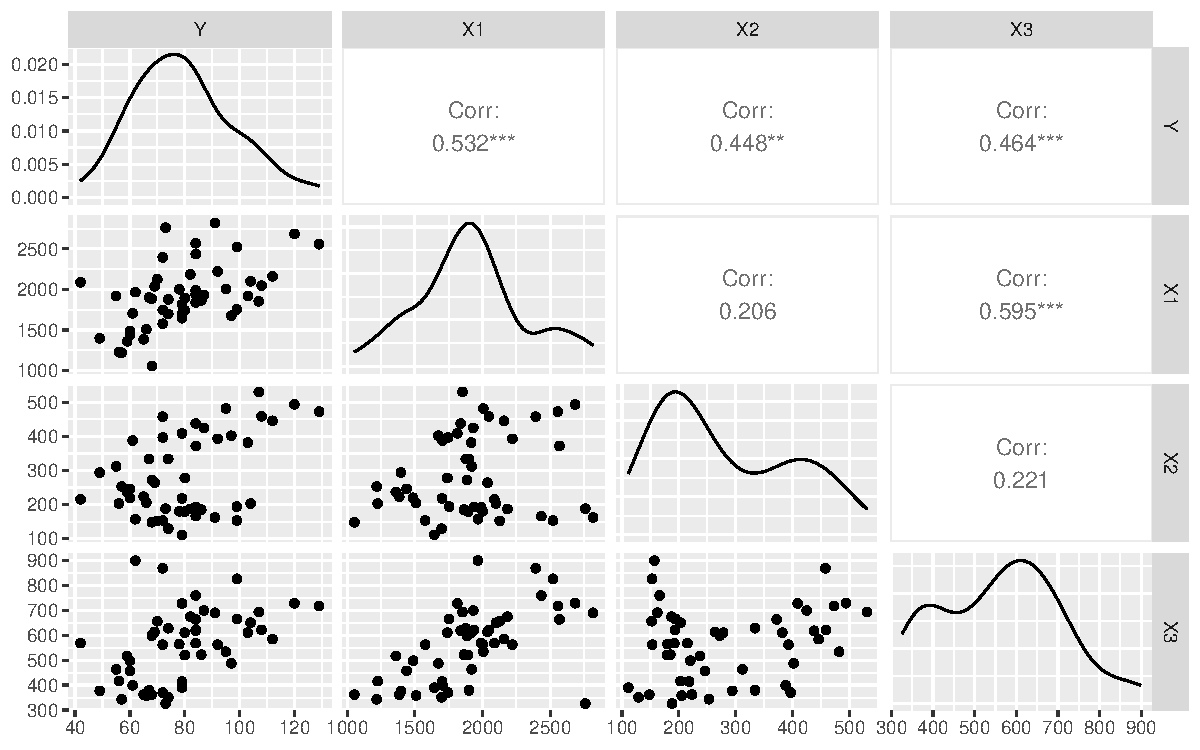
\includegraphics[width=.75\textwidth]{pair_plot.pdf}
\end{figure}

Alternatively, we can create 6 scatterplots, and combine them into one plot. As this is a tedious task. I will include the code for \textbf{1 Plot} and the combination into one plot.

\lstinputlisting[language = R, firstline = 152, lastline = 159]{PS01_AL.R}
\lstinputlisting[language=R, firstline = 217, lastline = 217]{PS01_AL.R}

\begin{figure}[h!]\centering
	\caption{\footnotesize Bivariate Correlations for Variable of Interest .}
	\label{fig:plot_2}
	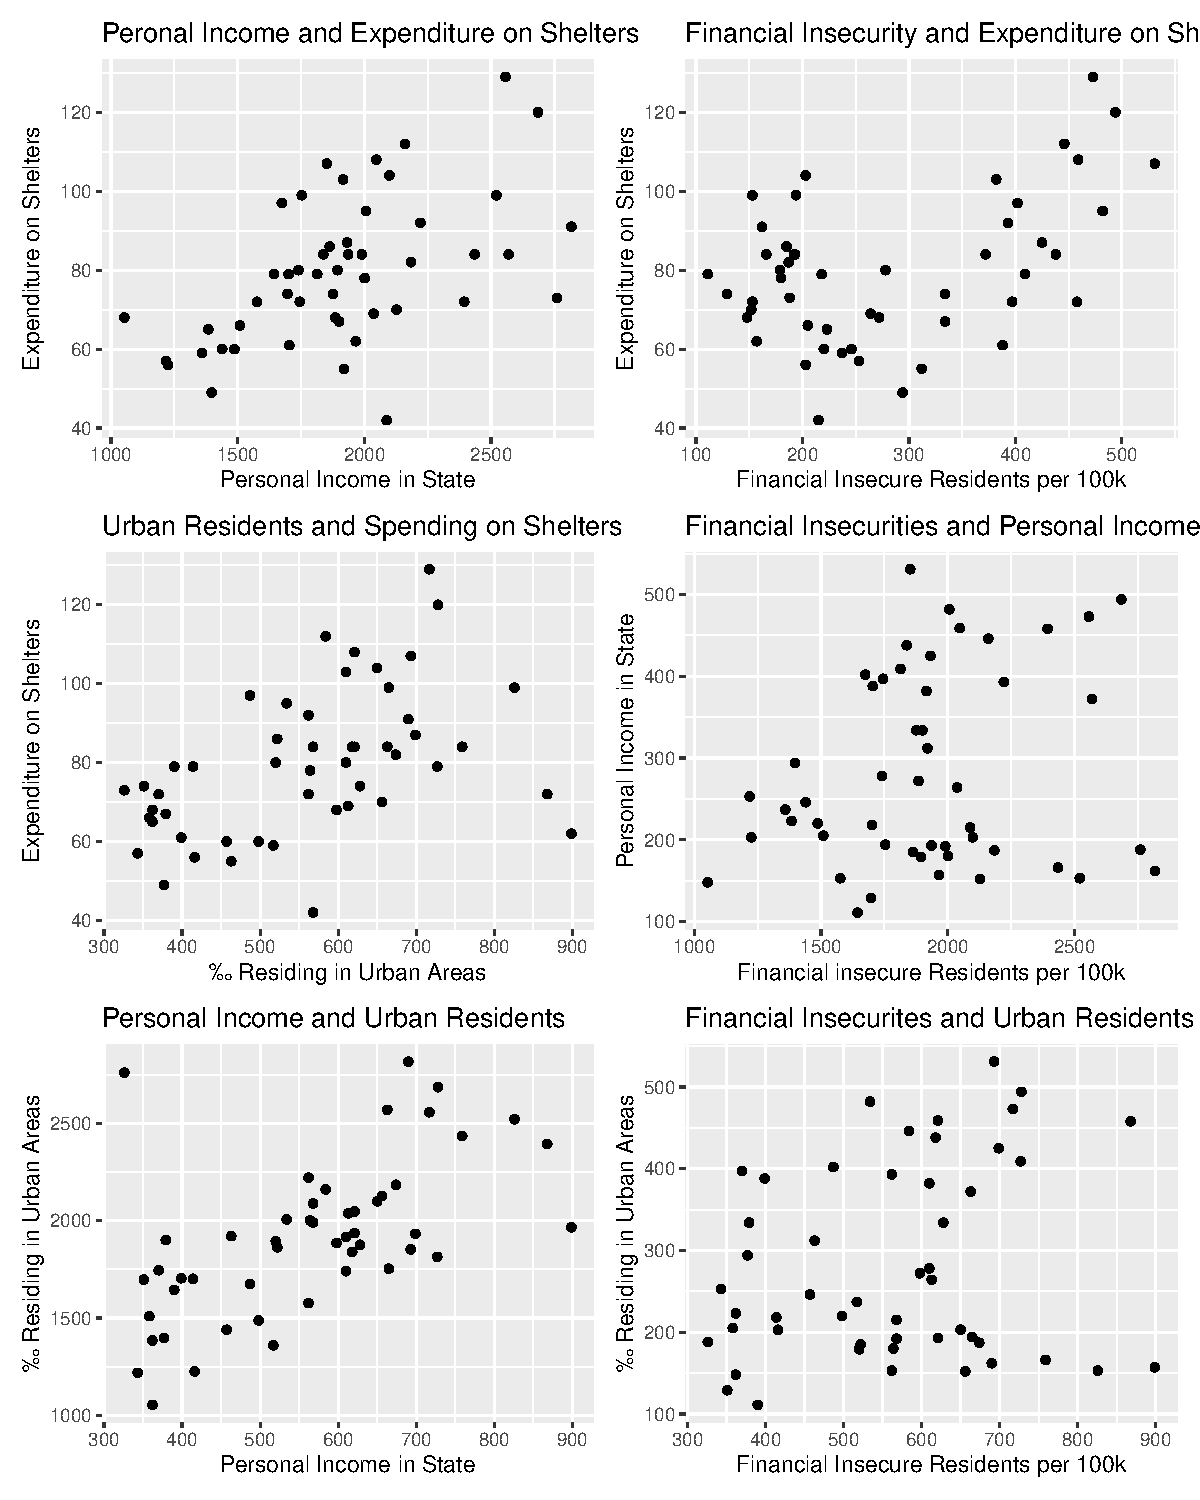
\includegraphics[width=.75\textwidth]{plot_combined.pdf}
\end{figure}

Based on the visual representation of the date, there seems to be a positive linear relationship between 
\begin{itemize}
	\item  The per capita personal income in a state \textbf{(X1)} and the per capita expenditure on shelters/housing assistance in the same state \textbf{(Y)}
	\item The portion of urban residents \textbf{(X3)} and the spending on shelters \textbf{(Y)}. However, there are to outliers with high portions of urban residents and love expenditure on shelters. These 2 observations may affect the correlation coefficent
	\item Person Income \textbf{(X1)} and the proportion of Urban Residents \textbf{(X3)} 
\end{itemize}

The relationships between the textit{Number of residents per 100,000 that are ”financially insecure” in state} on the one hand side, and Personal Income per Capita, respectively protion of Urban Residents on the other hand's side are less clear. Based on the visual information from the plots, I would suggest they are positvely correlated. But the magnitude should be rather small, as there is no clear \textbf{linear} association

The relationship between residents with fianancial insecurities and Expenditure seems to be j-shaped. Again, I would suggest that this pattern hints at positive, but weak linear association.

Looking at the correlation coefficents from the \textbf{pair plot} 
We can see, that indeed, the correlation between \textbf{Y}, \textbf{X1}, and \textbf{X3} are the highest.
However, the relationshp between Y and X2 is only marginally smaller ($r = 0.448$). I would have expected a smaller value, considering, the j-spahed nature of the association.

The two remaining correlation coefficent \textbf{X2} with \textbf{X1}, and \textbf{X3} respectively, are somewhat smaller. This aligns well with the visual inspections.

\newpage
\item
Please plot the relationship between \emph{Y} and \emph{Region}? On average, which region has the highest per capita expenditure on housing assistance?
\vspace{.5cm}

\lstinputlisting[language = R, firstline = 229, lastline = 240]{PS01_AL.R}

\begin{figure}[h!]\centering
	\caption{\footnotesize Expenditure compared over Regions.}
	\label{fig:plot_3}
	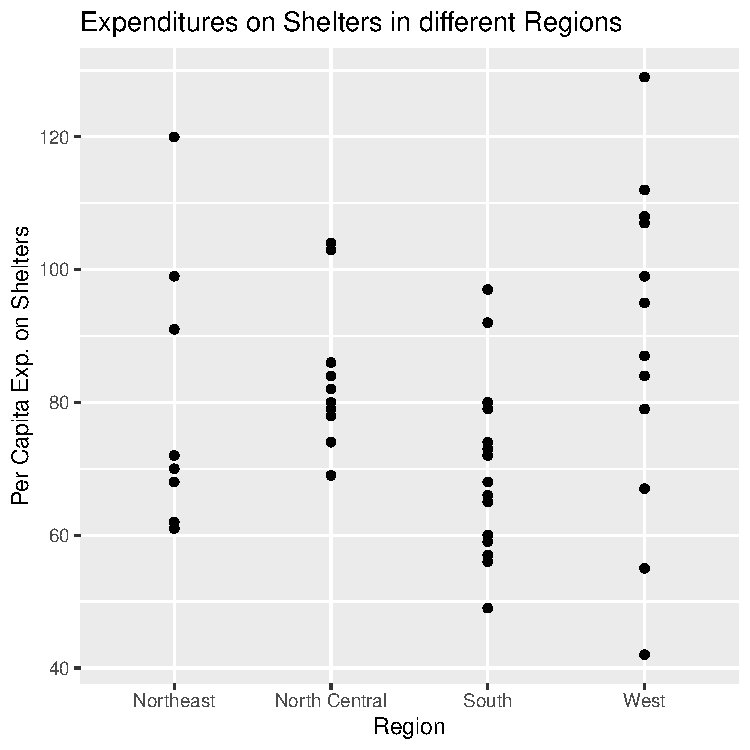
\includegraphics[width=.75\textwidth]{regions_plot.pdf}
\end{figure}

Based on the plot, I  would suggest that the Western Region has the highest average spending on housing assistance per capita 
However, based on the visual, I could not certainly differentiate between the other three regions. 
Furthermore, I run the numbers:

\begin{verbatim}
	> expenditure %>%
	+   dplyr::mutate(Region = factor(Region,
	+                                 levels = c(1, 2, 3, 4),
	+                                 labels = c("Northeast",
	+                                            "North Central",
	+                                            "South",
	+                                            "West"))) %>%
	+   dplyr::group_by(Region) %>%
	+   dplyr::summarise(mean_expenditure = mean(Y))
	# A tibble: 4 × 2
	Region        mean_expenditure
	<fct>                    <dbl>
	1 Northeast                 79.4
	2 North Central             83.9
	3 South                     69.2
	4 West                      88.3
\end{verbatim}

The output confirms my interpretation of the plot.


\item
Please plot the relationship between \emph{Y} and \emph{X1}? Describe this graph and the relationship. Reproduce the above graph including one more variable \emph{Region} and display different regions with different types of symbols and colors.
\end{itemize}

The code for the plot

\lstinputlisting[language=R, firstline = 273, lastline = 288]{PS01_AL.R}

\begin{figure}[h!]\centering
	\caption{\footnotesize Three Variable Plot.}
	\label{fig:plot_4}
	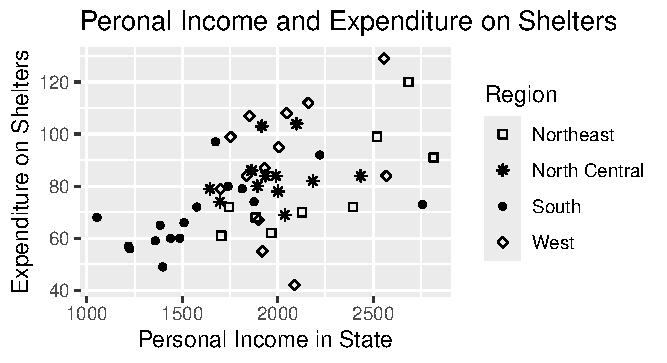
\includegraphics[width=.75\textwidth]{3var_plot.pdf}
\end{figure}

\end{document}
